%!TEX root = U-Wert.tex
%Einbindung Pakete
\documentclass[11pt,a4paper,oneside]{scrartcl}

%Pakete

%Style
\usepackage[left=2.5cm,right=2.5cm,top=2.0cm,bottom=2.5cm,footskip=1.5cm,head=25pt]{geometry}		
\usepackage{setspace}
\usepackage[bottom,hang]{footmisc}
\usepackage{longtable}

%Sprache
\usepackage[T1]{fontenc}  
\usepackage[utf8]{inputenc}
\usepackage[ngerman]{babel}
\usepackage{eurosym}
\usepackage{lmodern}
\usepackage{blindtext}

%Mathe- Umgebung
\usepackage{amsmath}
\usepackage{amssymb}
\usepackage{amsfonts}

%Grafiken
\usepackage{graphicx}																								
\usepackage{psfrag}
\usepackage{wrapfig}
\usepackage{subcaption}
\usepackage[headsepline,automark]{scrlayer-scrpage}

%Tabellenstil
\usepackage{tabularx}
\usepackage{multirow}
\usepackage{booktabs}
\usepackage{colortbl}
\usepackage[xcdraw]{xcolor}

%Referenzen
\usepackage{url}
\usepackage{hyperref}
\bibliographystyle{unsrt}

%Das hyperref paket führt zu Problemen mit der Internet-Link Darstellung, da bei diesen mit aktivem Paket kein Zeilenumbruch möglich ist ggf. kann hier eine eigene Lösung gefunden werden
%\usepackage[hidelinks]{hyperref}

%Grafikpafad
\graphicspath{{./Abbildungen/}}

%Zusätzliche Pakete
\usepackage{caption}
\usepackage{units}
\usepackage{float}
\usepackage[]{xcolor}
\usepackage{colortbl}
\usepackage{hhline}

%Nachträglich hinzugefügte Pakete
%\usepackage{auto-pst-pdf}


%Initialisierung des Dokuments
\begin{document}

%Einbindung unterschiedlicher Befehlsänderungen
%  Referenzen Befehle
\newcommand{\fref}[1]{Abb. \ref{fig:#1}}
\newcommand{\tref}[1]{Tab. \ref{tab:#1}}
\newcommand{\mref}[1]{(\ref{eq:#1})}
\newcommand{\sref}[1]{Abschnitt \ref{section:#1}}

%Kopfzeile
\ohead[{
\includegraphics[height=20pt]{HTWLogo}}]{
\includegraphics[height=20pt]{HTWLogo}}
\renewcommand*\sectionmarkformat{}

%Farbe
\definecolor{HTWGreen}{cmyk}{0.55, 0.00, 1.00, 0.00}

%Nachträglich hinzugefügte Style Änderungen und Befehlsänderungen



\parindent 0cm

%Zeilenabstand	
\onehalfspacing			 									
\addtolength{\footskip}{-8mm}

%Titelseite
\begin{titlepage}

		\begin{figure}[h] 
				\begin{flushright}
			
\includegraphics[width=0.3\textwidth]{HTWLogo}\\
				\end{flushright}
		\end{figure}
		
%Hochschulspezifische Informationen, Hochschule, Fachbereich, Adresse, etc.
	\begin{center}
		\vspace*{\fill}
		{\Large Hochschule f{\"u}r Technik und Wirtschaft Berlin}\\
			\bigskip
			Wilhelminenhofstra"se 75A, 12459 Berlin\\
			\bigskip
		Fachbereich 1 \\Ingenieurwissenschaften - Energie und Information\\Regenerative Energien (B)\\
		\vfill
%Versuchspezifische Angaben
		 \textcolor{HTWGreen}{\textbf{\Large{Brennstoffzellenversuch vom 16.06.2023}}}\\
		\textit{Betreuer*in: M.Sc. Sabine Kupzok}\\
		\textit{Gruppe: 5}\\
	\vfill
	\end{center}
\vfill
%Gruppenmitglieder Liste
\begin{table}[H]
			\centering
			\begin{tabular}{|l|c|}
			\hline
			\rowcolor[cmyk]{0.55, 0.00, 1.00, 0.00} \textbf{Name} & \textbf{Matrikelnummer}  \\
			\hline
			Johannes Tadeus Ranisch     & 578182\\
			\hline
			Markus Jablonka       & 580234\\
			\hline
			Niels Feuerherdt      & 577669\\
			\hline
			Katharina Jacob			 & 578522\\
			\hline
			Lukas Aust			 & 574051\\
			\hline
			\end{tabular}
			\end{table}
\end{titlepage}

\newpage

%Abstract (dieser ist für Labor Protokolle in der Regel nicht notwendig)
%\begin{abstract}

\begin{center}
\normalsize \textbf{Abstract}\\
\end{center}

\noindent
Kurze Zusammenfassung der Ergebnisse des Versuchs. Dieser wird in der Regel zuerst gelesen um zu identifizieren ob die vorliegende Arbeit Informationen enthält nach denen der Leser sucht.



\end{abstract}
\newpage

\pagenumbering{roman}

%Inhaltsverzeichnis
\setcounter{tocdepth}{2}
\tableofcontents
\newpage

%Abbildungsverzeichnis, Tabellenverzeichnis und Abkürzungsverzeichnis
\listoffigures
\listoftables
\addtocounter{table}{-1} 
\bigskip
\Large \textsf{\textbf{Abk"urzungsverzeichnis}}
\begin{longtable}{p{2 cm}p{8 cm}} 
\end{longtable}
\newpage

\pagenumbering{arabic}

%Inhaltlicher Teil
\section{Versuchsziele}
\begin{figure}[!h]
		\centering
		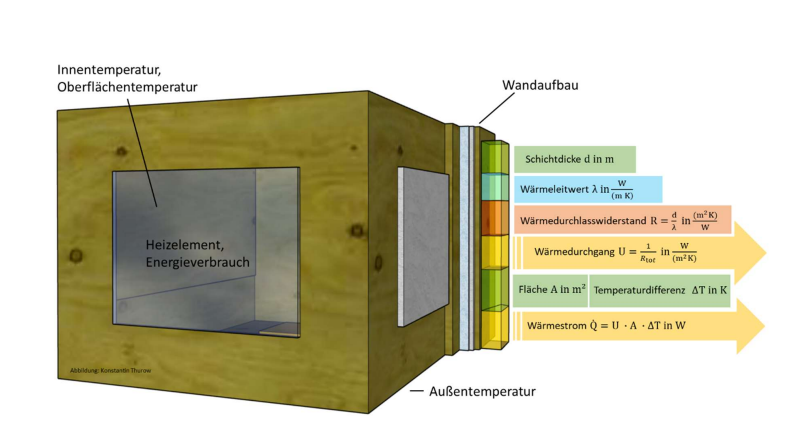
\includegraphics[width=0.7\textwidth]{Abbildungen/Thurow_Deckblatt}
		\caption{Animation des Versuchsaufbaus [Versuchsanleitung] }
		\label{fig:Versuchsaufbau}
\end{figure}

Mit Blick auf die Ziele der Bundesregierung den Endenergieverbrauch bis 2030 um 24\% zu senken gewinnt Energieeffizienz im Bausektor mit rasender Geschwindigkeit an Relevanz. Die Effizienzklassen für Neubauten legen den Fokus auf Dämmungen und können so in den nächsten Jahrzehnten viel Gas und Kohle einsparen. Dieser Versuch soll ein Versändnis für Dämmstoffe und die Klassifikation dieser durch den Wärmedurchgangskoeffizienten (U-Wert) schaffen.  Der Versauchsaufbau besteht aus einem Modellhaus (\autoref{fig:Versuchsaufbau}) austauschbaren Wänden , einem abnehmbaren Dach und einer Glühlampe als Wärmequelle. Ziel ist es aus den aufgenommenen Temperaturdifferenzen in der Auswertung die Wärmeleitfähigkeit und den Wärmedurchgang der einzelnen Materialien zu bestimmen.\\\\
Aus Erfahrungswerten und bisherigen Vorlesungsveranstaltungen lässt sich vermuten, dass einige der Materialien Wärme besser leiten als andere. Während Polysterol, oftmals auch als Dämmstoff genutzt, eine schlechte Wärmeleitfähigkeit aufweisen wird, leitet das Floatglas Wärme wahrscheinlich am besten und hat so auch den größten U-wert. Erwartbar ist außerdem, dass die U-werte in der zweiten Messung geringer sein werden als in der ersten da das Schichtholz durch eine Dämmung ergänzt wurde.
\newpage
\section{Vorbereitungsfragen}
\subsection{1}
\begin{figure}[H]
    \centering
    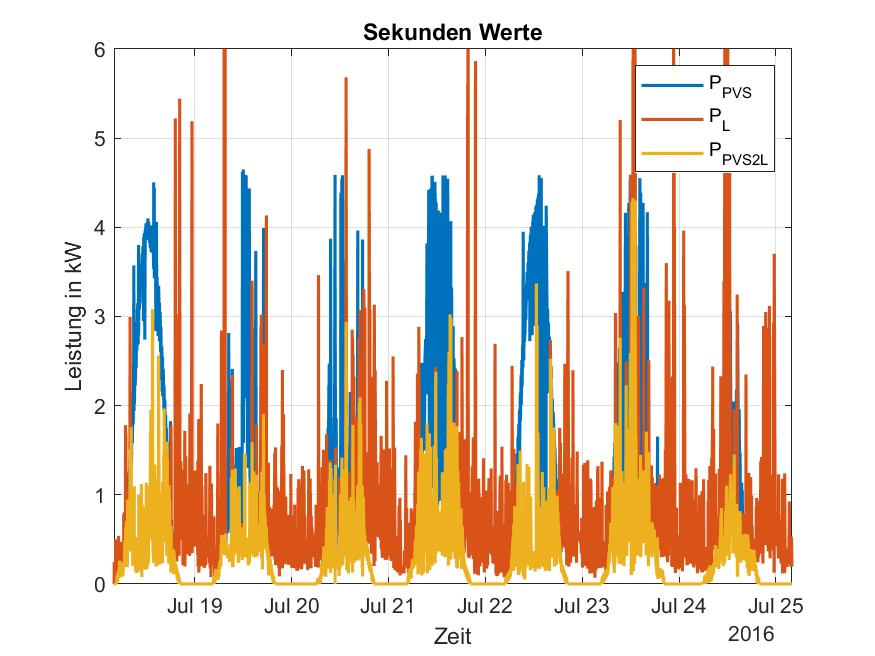
\includegraphics[width=\textwidth]{Abbildungen/plot.jpg}
    \caption{Beschreibung des Plots}
    \label{fig:plot3062023}
\end{figure}
\subsection{2}
$E.E_pvs = sum(ts.Ppvs/1000)/3600=149,96kWh;\\
E.E_l = sum(ts.Pl/1000)/3600=89,08kWh;\\
E.E_pvs2l = sum(Ppvs2l/1000)/3600=41,52kWh;$\\

\subsection{3}
\begin{figure}[H]
    \centering
    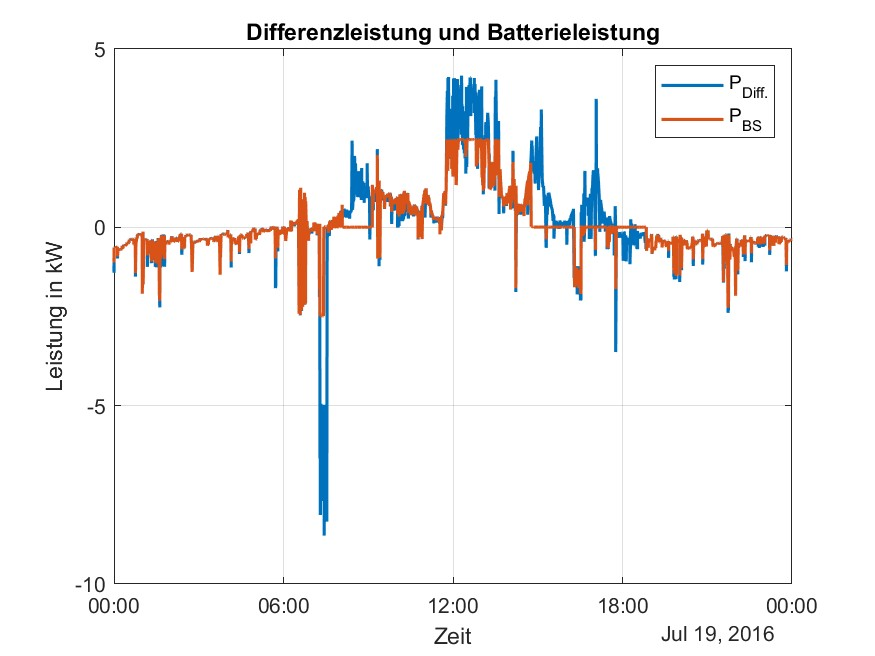
\includegraphics[width=\textwidth]{Abbildungen/plot_vorbereitungsfrage3.jpg}
    \caption{Beschreibung des Plots}
    \label{fig:plot3062023}
\end{figure}
\subsection{4}
\begin{figure}[H]
    \centering
    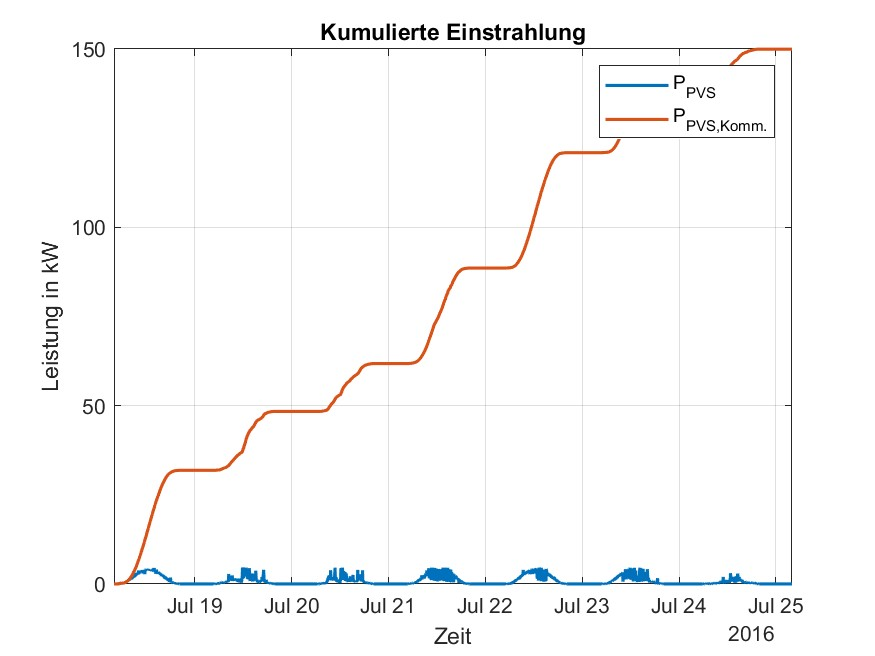
\includegraphics[width=\textwidth]{Abbildungen/plot_vorbereitungsfrage4.jpg}
    \caption{Beschreibung des Plots}
    \label{fig:plot43062023}
\end{figure}
Der MATLAB-Befehl cumsum steht für cumulative sum und wird verwendet, um die kumulative Summe eines Vektors oder einer Matrix zu berechnen. 
Also statt die gesammte Summe zu berechnen, werden mit cumsum auch alle zwischen Summen gespeichert. In \autoref{fig:plot43062023} ist zu sehen, wie mit Hilfe des Befehls die Leistungen kummuliert werden und man eine Aussage über die kummulierte Einstrahlung erhält.
\section{Auswertung}
\label{sec:Auswertung}
\subsection{Energiebilanz der Anlage und äußere Leistungszahl}
In diesem Teil werden die Leistungszahlen und die Energiebilanz der Anlage berechnet.

\subsubsection{Prüfung Heizleistung}
\label{subsubsec:Heizleistung}
anhand von Heizdurchfluss, Vor- und Rücklauftemperatur
Die Heizleistung oder auch Heizdurchfluss wird mit der \autoref{eq:110623_Heizleistung} berechnet:

\begin{equation}
\dot Q_{Kond}= \dot m \cdot cp_{W} \cdot (T_{V} - T_{R})
\label{eq:110623_Heizleistung}
\end{equation}

Im ersten Schritt wird der Massenstrom über den Volumenstrom nach \autoref{eq:230624_Massestrom_V_D} bestimmt werden.

\begin{equation}
    \dot{m}= \dot{V}\cdot \rho
    \label{eq:230624_Massestrom_V_D}
\end{equation}

$$\dot{m}= 0,391 \cdot 10^{-3}\frac{m^3}{s} \cdot 990 \frac{kg}{m^3}=0,38 \frac{kg}{s}$$

Mithilfe dieses Massenstroms kann die Heizleistung berechnet werden.

$$\dot Q_{Kond}= 0,38 \frac{kg}{s} \cdot 4,2 \frac{kJ}{kg \cdot K} \cdot (48 ^{\circ}C - 43 ^{\circ}C) = 8,14 \frac{kJ}{s}$$

Mit einem Massenstrom von 0,38 $\frac{kg}{s}$, einer Vorlauftemperatur von 48 °C und Rücklauftemperatur von 43 °C im Kondensator ergibt sich daraus mit Formel \ref{eq:110623_Heizleistung} eine Heizleistung von 8,14 $\frac{kJ}{s}$ bzw $kW$. Wobei auf dem Display eine Heizleistung von 8,3kW angezeigt wird, was nur minimal vom errechneten Wert abweicht.
\subsubsection{Äußere Leistungszahl}
Die tatsächliche äußere Leistungszahl berechnet sich wie in Formel \ref{eq:110623_aeußere Leistungszahl_tatsächlich} dargestellt und beträgt 3,54.

\begin{equation}
\epsilon_{Real,Au"sen} = \frac{\dot Q_{Nutz}}{P_{el}}
\label{eq:110623_aeußere Leistungszahl_tatsächlich}
\end{equation}

$$ \epsilon_{Real,Au"sen} = \frac{8,14 kW}{2,3 kW} = 3,54$$

\subsubsection{Wärmestrom im Verdampfer aus Gesamt-Energiebilanz}
Um den aus der Umgebung aufgenommenen Wärmestrom zu bestimmen, muss die Gesamt-Energiebilanz der Anlage verwendet werden:

\begin{equation}
\dot Q_{Verd}=\dot Q_{Kond}-P_{el}
\label{eq:110623_aeußere Leistungszahl}
\end{equation}

$$\dot Q_{Verd}= 8,14 kW-2,304 kW= 5,84kW $$


Mit der berechneten Heizleistung von 8,14kW und einer elektrischen Leistung von 2304W ergibt sich ein vom Verdampfer aufgenommenen Wärmestrom von 5,84kW. Nun wird der benötigte Luftstrom, unter der Annahme, dass die durchströmende Luft um 5K abgekühlt wird, berechnet.

Welcher Luftvolumenstrom muss durchgesetzt werden, wenn die Luft um 5 K abgekühlt wird?
\begin{equation}
\dot V_{L}=\frac{\dot Q_{verd}}{\rho_{Luft} \cdot cp_{Luft} \cdot \Delta T}
\label{eq:110623_benoetigter_Luftstrom}
\end{equation}

$$\dot V_{L}=\frac{5,84 kW}{ 1,2 \frac{kg}{m^3} \cdot 1 \frac{kJ}{kg \cdot K} \cdot 5K}= 0,973 \frac{m^3}{s}$$


Der benötigte Luftstrom beträgt nach Formel \ref{eq:110623_benoetigter_Luftstrom} 0,973$\frac{m^3}{s}$. 
\subsubsection{Äußere Carnot-Leistungszahl der Anlage \texorpdfstring{$\epsilon_{Carnot,a}$}{}}
\label{subsubsec:Carnot}

Für die äußere Carnot-Leistungszahl der Anlage wird die Umgebungstemperatur $T_{U}=$24°C= 297,15K und die mittlere Temperatur der Nutzwärme benötigt.

\begin{equation}
T_{mN}= \frac{T_{Kessel}+T_{Rück}}{2}
\end{equation}

$$T_{mN}=\frac{51,6^{\circ}C+44,9^{\circ}C}{2}=48,25^{\circ}C= 321,4 K$$

Die äußere Carnot-Leistungszahl berechnet sich dann wie folgt: 

\begin{equation}
\epsilon_{Carnot, Au"sen} = \frac{T_{mN}}{T_{mN}-T_{U}}
\label{eq:110623_aeußere Carnot Leistungszahl}
\end{equation}

$$\epsilon_{Carnot, Au"sen} = \frac{321,4 K}{321,4 K-297,15K} = 13,25$$

Sie beläuft sich dabei auf 13,25.

\subsection{Arbeitsmittelkreislauf und innere Leistungszahlen}
Entsprechend der Werte aus Messreihe 1, welche in \autoref{tab:Arbeitspunkte} zusammengefasst sind, kann das passende
lg(p)-h-Diagramm, mit den Arbeitspunkten 1-4 erstellt werden. Aus diesem Diagramm lassen sich die in \autoref{tab:Arbeitspunkte} ebenfalls
notierten Enthalpien ablesen.

\begin{table}[!ht]
    \centering
    \resizebox{\textwidth}{!}{%
    \begin{tabular}{|c|c|c|c|}
        \hline
        \rowcolor[HTML]{70AD47} 
        \multicolumn{1}{|l|}{\cellcolor[HTML]{70AD47}{\color[HTML]{000000} \textbf{Arbeitspunkt}}} & {\color[HTML]{000000} Bezeichnung} & \multicolumn{1}{l|}{\cellcolor[HTML]{70AD47}{\color[HTML]{000000} Temperatur in °C}} & \multicolumn{1}{l|}{\cellcolor[HTML]{70AD47}{\color[HTML]{000000} Enthalpie in kJ/kg}} \\ \hline
        \rowcolor[HTML]{CFE5A8} 
        1                                                                                          & Temperatur nach Verdampfer         & 18                                                                                   & 425                                                                                    \\ \hline
        \rowcolor[HTML]{E2EFDA} 
        2                                                                                          & Heißgastemperatur                  & 66                                                                                   & 453                                                                                    \\ \hline
        \rowcolor[HTML]{CFE5A8} 
        3                                                                                          & Verflüssigertemperatur             & 45                                                                                   & 276                                                                                    \\ \hline
        \rowcolor[HTML]{E2EFDA} 
        4                                                                                          & Temperatur vor Verdampfer          & 15                                                                                   & 276                                                                                    \\ \hline
        \end{tabular}%
    }
    \caption{Arbeitspunkte entsprechend Messreihe 1}
    \label{tab:Arbeitspunkte}
    \end{table}

    \begin{figure}[!ht]
        \centering
        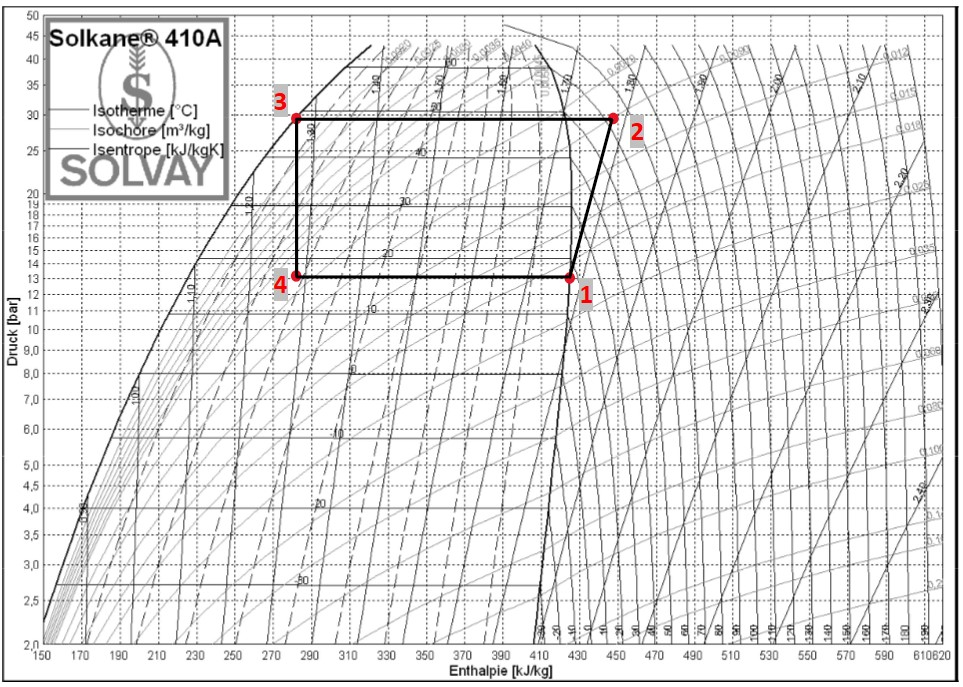
\includegraphics[width=\textwidth]{Abbildungen/lgp-h-diagramm.jpg}
        \caption{lg(p)-h-Diagramm für den realen Kreisprozess mit Darstellung der Irreversibilität}
        \label{fig:lgp-h-Diagramm}
    \end{figure}


    Zusätzlich kann das obere Druckniveau von 28 bar und das unter Druckniveau von rund 12,8 bar abgelesen werden.
    Des Weiteren ist in \autoref{fig:lgp-h-Diagramm} ersichtlich, dass die Ergebnisse plausibel sind, da der dargestellte Kreisprozess dem erwarteten Bild entspricht. Einzig der minimale Anstieg der Temperatur von Punkt 4 zu Punkt 1 ist ungewöhnlich, allerdings durch einfache Fehler beim Messen oder Verluste am Verdampfer zu erklären.\\

Mit den Temperaturen aus \autoref{tab:Arbeitspunkte} kann mittels \autoref{eq:Innere Carnot-Leistungszahl} die innere Carnot-Leistungszahl
ermittelt werden. Die Berechnung ergibt dann eine innere Carnot-Leistungszahl von 10,605.

    \begin{equation}
        \epsilon_{Carnot, Innen}=\frac{T_{max}}{T_{max}-T_{min}}=\frac{T_{Kond}}{T_{Kond}-T_{Verd}}
        \label{eq:Innere Carnot-Leistungszahl}
    \end{equation}

$$\epsilon_{Carnot, Innen}=\frac{318,15 K}{318,15 K-288,15 K}=10,605$$

 In \autoref{fig:lgp-h-Diagramm} ist zusätzlich der isentrope Arbeitspunkt 2 eingezeichnet und somit ist eine isentrope Enthalpie für diesen Arbeitspunkt von $445 \frac{kJ}{kg}$abzulesen.
Mittels der nun bekannten isentropen Enthalpie für Arbeitspunkt 2 kann mittels \autoref{eq:Isentropenwirkungsgrad} der Isentropenwirkungsgrad ermittelt werden.
\begin{equation}
    \eta_{is}=\frac{h_{2,is}-h_{1}}{h_{2}-h_{1}}
    \label{eq:Isentropenwirkungsgrad}
\end{equation}

$$\eta_{is}=\frac{(445-425)\frac{kJ}{kg}}{(453-425)\frac{kJ}{kg}}=0,714$$

Der Isentropenwirkungsgrad für diesen Fall beträgt demnach 0,714.\\


\subsubsection{Innere Leistungszahlen}

\begin{equation}
   \epsilon_{VP,i} = \frac{h_{2,is}-h_{pH}}{h_{2,is}-h^{''}_{p0}}
\label{eq:230623_Leistungszahl_VPI}
\end{equation}

Aus der Dampftafel für das Kältemittel R410a wurden die Werte $h"_{p0}=425,46 \frac{kJ}{kg}$ und $h_{pH}= 225,03 \frac{kJ}{kg}$ entnommen und mit den Werten aus \autoref{tab:Arbeitspunkte} in \autoref{eq:230623_Leistungszahl_VPI} eingesetzt
$$\epsilon_{VP,i} = \frac{h_{2,is}-h_{pH}}{h_{2,is}-h^{''}_{p0}}$$

\begin{equation}
    \epsilon_{real,i}= \frac{h_2-h_3}{h_2-h_1}
\end{equation}
$$\epsilon_{VP,i}= \frac{(453-275,84)\frac{kJ}{kg}}{(453-425,46)\frac{kJ}{kg}} = 6,433 $$
$$\epsilon_{real,i}= \frac{(453-276)\frac{kJ}{kg}}{(453-425)\frac{kJ}{kg}} = 6,321 $$

\subsection{Leistungszahlen und Verlustursachen}

% Leistungszahl auflistung nach finalisierung von Niels und Lukas

$$\epsilon_{Carnot,Au"sen} = 13,25$$
$$\epsilon_{Carnot,Innen} = 10,605$$
$$\epsilon_{VP,Innen} = 6,433$$
$$\epsilon_{Real,Innen} = 6,321$$
$$\epsilon_{Real,Au"sen} = 3,54$$

\begin{table}[!ht]
    \centering
    \caption{Leistungszahlen in absteigender Reihenfolge}
    \label{tab:Leistungszahlen}
    \begin{tabular}{|l|l|l|}
        \hline
    \rowcolor[HTML]{70AD47} 
    {\color[HTML]{333333} \textbf{Leistungszahl}}  & {\color[HTML]{333333} \textbf{Wert}} & {\color[HTML]{333333} \textbf{Differenz}} \\
    \rowcolor[HTML]{C6E0B4} 
    $\epsilon_{Carnot,Au"sen}$ & 13,25                                & 0                                         \\ \hline
    \rowcolor[HTML]{E2EFDA} 
    $\epsilon_{Carnot,Innen}$  & 10,605                               & 2,645                                     \\ \hline
    \rowcolor[HTML]{C6E0B4} 
    $\epsilon_{VP,Innen}$      & 6,433                                & 4,172                                     \\ \hline
    \rowcolor[HTML]{E2EFDA} 
    $\epsilon_{Real,Innen}$    & 6,321                                & 0,112                                     \\ \hline
    \rowcolor[HTML]{C6E0B4} 
    $\epsilon_{Real,Au"sen}$   & 3,54                                 & 2,781                                     \\ \hline
    \end{tabular}%
    \end{table}

Wie ersichtlich ist, gibt $\epsilon_{Carnot,Au"sen}$ die maximale Leistungszahl an. 
Dies liegt daran, dass der äußere Carnot-Wirkungsgrad einen idealisierten Prozess darstellt, bei dem Verluste vollständig vernachlässigt werden. 
Er vergleicht lediglich die Temperaturänderung der mittleren Nutzwärme mit der Umgebungstemperatur.

Der äußere Carnot-Wirkungsgrad ist größer als der innere Carnot-Wirkungsgrad $\epsilon_{Carnot,Innen}$, da sich der innere auf die Kondensations- und Verdampfungstemperatur stützt. 
Um die Wärme auf den Prozess zu übertragen und wieder abzugeben, sind Temperaturunterschiede an den beiden Wärmetauschern erforderlich. 
Bei der Wärmepumpe erfolgt die Wärmeübertragung am Verdampfer und am Kondensator. 
Diese Verluste der Wärmeübertragung werden beim inneren Carnot-Wirkungsgrad berücksichtigt.

Die innere Leistungszahl für den Vergleichsprozess $\epsilon_{VP,Innen}$ wurde mithilfe der theoretischen Enthalpien des Kältemittelkreislaufs berechnet.
Dies sind abgelesene Werte aus Diagrammen oder Tabellen und können daher etwas ungenauer sein. 
Der theoretische Carnot-Prozess zur allgemeinen Wärmeübertragung wird nun durch einen realen Kältemittelkreislauf realisiert. 
Das Kältemittel Solkane 410A weist stoffspezifische Enthalpien auf. 
Dadurch entstehen Verluste aufgrund des Stoffs und der tatsächlichen Prozessführung.

Als vorletzte Leistungszahl haben wir die reale innere Leistungszahl $\epsilon_{Real,Innen}$.
Diese ist geringer, da die Übergänge im realen Verlauf nicht isentrop, sondern irreversibel sind. 
Die Druck- und Reibungsverluste einzelner Bauteile werden nun berücksichtigt. 
Der Verdampfer sollte das Arbeitsmittel leicht überhitzen, da es sonst bereits in der Leitung zum Verdichter kondensieren könnte. 
Außerdem findet die Wärmezufuhr nicht wie theoretisch berechnet isobar statt.

Die Verdichtung weist Verluste auf und erfolgt nicht isentrop.

Im Kondensator ist das Arbeitsmittel überhitzt und gibt daher Wärme bei einer höheren Temperatur als der Kondensationstemperatur ab. 
Dadurch entstehen Wärme- und Druckverluste, ähnlich wie im Verdampfer. 
Die Kondensation findet ebenfalls aufgrund der Verluste nicht isobar statt.
und auch die  Drossel arbeitet effizient, aber nicht perfekt isenthalp.
\\
Die geringste Leistungszahl weist die äußere Leistungszahl $\epsilon_{Real,Au"sen}$ auf. 
Dieser Wert berücksichtigt den tatsächlich benötigten Nutzwärmestrom und die dafür erforderliche elektrische Verdichterleistung. 
Er umfasst daher alle Verluste im gesamten System.


\subsection{Energiebilanzen Einzelapparate}
\label{subsec:Massenstrom}
\subsubsection{Arbeitsmittelmassenstrom Kondensator/Verdampfer}
\begin{equation}
   \dot m_{AM} = \frac{\dot Q_{Kond}}{|(h_3 - h_2)|}
   \label{eq:230623_massestrom}
\end{equation}
Mit $\dot Q_{Kondensator}=8,14kW$, $h_2=453\frac{kJ}{kg}$ und $h_3=276\frac{kJ}{kg}$ wird der Massenstrom des Kondensators nach \autoref*{eq:230623_massestrom} berechnet:

$$ \dot m_{AM_{Kond}} = \frac{8,14kW}{|(276\frac{kJ}{kg} - 453\frac{kJ}{kg})|} = 0,04746 \frac{kg}{s} $$

\begin{equation}
  \dot m_{AM_{Verd}} = \frac{\dot Q_{Verd}}{|(h_1-h_4)|}
    \label{eq230623_massestrom_ver}
\end{equation}

Mit $\dot Q_{Verd}=5,84kW$, $h_1=425\frac{kJ}{kg}$ und $h_4=276\frac{kJ}{kg}$ wird der Massenstrom des Kondensators nach \autoref*{eq230623_massestrom_ver} berechnet:
$$\dot m_{AM} = \frac{5,84 kW}{|(425\frac{kJ}{kg}-276\frac{kJ}{kg})|} = 0,03907 \frac{kg}{s}$$

$$\overline{\dot m}_{AM} = \frac{\dot m_{AM_{Kond}}+\dot m_{AM_{Verd}}}{2} = \frac{0,04746 \frac{kg}{s}+0,03907 \frac{kg}{s}}{2} = 0,04327 \frac{kg}{s} $$



\subsubsection{Verdichterleistung und Verdichterwirkungsgrad}

Die Verdichterleistung wird als mechanische Leistung nach \autoref{eq:230623_Verdichterleistung} berechnet.

\begin{equation}
    P_{mech} = \overline{\dot m}_{AM} \cdot (h_2-h_1)
\label{eq:230623_Verdichterleistung}
\end{equation}
$$  P_{mech} = 0,04327 \frac{kg}{s} \cdot (453-425)\frac{kJ}{kg} = 1,211 kW $$

\begin{equation}
  \eta_{Ver} = \frac{P_{mech}}{P_{el}}=\frac{\overline{\dot m}_{AM}\cdot (h_2-h_1)}{P_{el}}=\frac{\overline{\dot m}_{AM}\cdot (h_2,is-h_1)}{P_{el}\cdot \eta_{is}}
\label{eq:230623_Verdichterwirkungsgrad}
\end{equation}

$$\eta_{Ver} = \frac{0,04327 \frac{kg}{s}\cdot (445-425)\frac{kJ}{kg}}{1,8 kW \cdot 0,714}= 0,6733 \approx 67,33 \% $$

\subsubsection{Strömungsgeschwindigkeiten von Gas und Flüssigkeit}

Das spezifische Volumen des Gases kann aus dem lg(p)-h-Diagramm in \autoref{fig:lgp-h-Diagramm} abgelesen werden zu: $V_{Gas}=0,019 \frac{m^3}{kg}$. Die Dichte, welches der Kehrwert des spezifischen Volumens ist, ergibt sich als $\rho=52,63 \frac{kg}{m^3}$. 
Mit dem durchschnittlichen Massenstrom aus \autoref{subsec:Massenstrom} können die Strömungsgeschwindigkeiten über den Volumenstrom nach folgenden Gleichungen berechnet werden.

\begin{equation}
    \dot{V}= \frac{\overline{\dot m}_{AM}}{\rho }
    \label{eq:230620_Volumenstrom}
\end{equation}

\begin{equation}
    \dot{V}= v \cdot \frac{\pi}{4} \cdot d^2
    \label{eq:230620_Volumenstrom2}
\end{equation}

Der Durchmesser der Heißgasleitung beträgt 16 mm, der der Kondensatleitung 10
mm.
Werden \autoref{eq:230620_Volumenstrom} und \autoref{eq:230620_Volumenstrom2} gleichgesetzt ergibt sich die Strömungsgeschwindigkeit nach \autoref{eq:230620_Strömungsgeschwindigkeiten}.

\begin{equation}
    v = \frac{\overline{\dot m}_{AM}}{\frac{\pi}{4}\cdot \rho \cdot d^2}
    \label{eq:230620_Strömungsgeschwindigkeiten}
\end{equation}

Am Arbeitspunkt 1 ist die Strömungsgeschwindigkeit:
$$v=\frac{0,04327 \frac{kg}{s}}{\frac{\pi}{4}\cdot 52,63 \frac{kg}{m^3} \cdot (0,016 m)^2}=4,089 \frac{m}{s} $$

Der Druck am Arbeitspunkt 3 kann aus dem lg(p)-h Diagramm als $p=28 bar$ abgelesen werden. Mit Hilfe dessen lässt sich die Dichte aus der Dampftafel als $\rho=935,99 kg/m^3$ bestimmen.
Die Strömungsgeschwindigkeit der Flüssigkeit am Arbeitspunkt 3 berechnet sich dann zu:
$$v=\frac{0,04327 \frac{kg}{s}}{\frac{\pi}{4}\cdot 935,99\frac{kg}{m^3} \cdot (0,01 m)^2}=0,588 \frac{m}{s}$$

\subsubsection{T,A-Schaubild des kleinen Gegenstrom-Plattenwärmeübertragers/K-Wert}

T,A-Schaubild des kleinen Gegenstrom-Plattenwärmeübertragers
zwischen internem und externem Heizkreis

\begin{figure}[!ht]
    \centering
    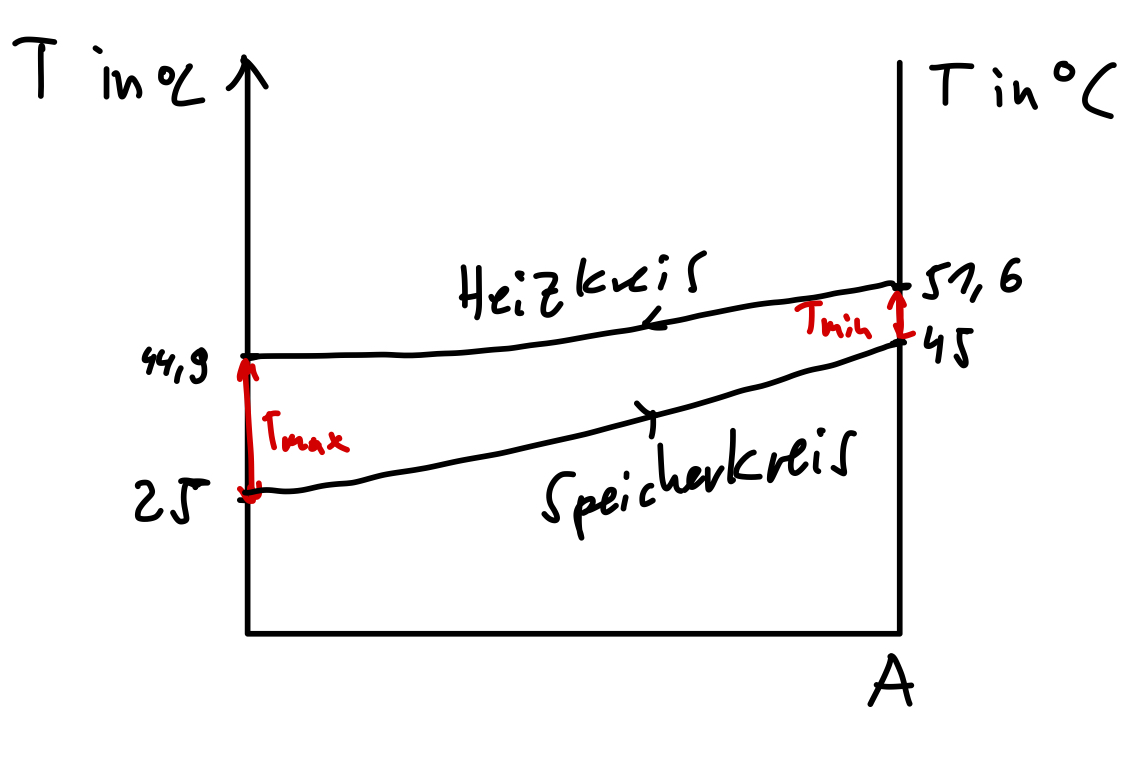
\includegraphics[width=0.5\textwidth]{Abbildungen/TA.Diagramm.jpeg}
    \caption{T,A-Schaubild eines Gegenstrom-Plattenwärmeübertragers}
    \label{fig:TA,Diagramm}
\end{figure}

\subsubsection*{K-Wert}
Für die Berechnung des K-Werts muss im Vorfeld $\Delta T_M$ bestimmt werden. Das passiert nach folgenden Gleichungen.

Die maximale Temperaturdifferenz wird aus der Speicher-Rücklauftemperatur und der Kesselrücklauftemperatur bestimmt.

\begin{equation}
    \Delta T_{MAX}= \Delta T_{HA}-\Delta T_{KE}
    \label{eq:230621_DeltaTMAX}
\end{equation}



$$\Delta T_{MAX}= 44,9\text{°}C-25 \text{°} C= 19,9K$$

Die minimale Temperaturdifferenz wird aus der Speicher-Vorlauftemperatur und der tatsächlichen Kesseltemperatur berechnet.

\begin{equation}
    \Delta T_{MIN}= \Delta T_{HE}-\Delta T_{KA}
    \label{eq:230621_DeltaTMIN}
\end{equation}

$$\Delta T_{MIN}= 51,6 \text{°} C-45 \text{°} C= 6,6K$$

\begin{equation}
    \Delta T_{M}= \frac{\Delta T_{MAX}-\Delta T_{MIN}}{ln(\frac{\Delta T_{MAX}}{\Delta T_{MIN})}}
    \label{eq:230621_DeltaTM}
\end{equation}

$$\Delta T_M= \frac{19,9K-6,6K}{ln(\frac{19,9K}{6,6K})}= 12,05K$$

Mithilfe der \autoref{eq:230621_Q}, der gegebenen Fläche von $A= 0,4m^2$ und der Heizleistung lässt sich der k-Wert bestimmen.

\begin{equation}
    \dot{Q}=k\cdot A \cdot \Delta T_M
    \label{eq:230621_Q}
\end{equation}

\begin{equation}
    k = \frac{\dot{Q}}{ A \cdot \Delta T_M} 
    \label{eq:230621_k}
\end{equation}

$$k=\frac{8,14 kW}{ 0,4m^2 \cdot 12,05K}=1,69 \frac{kW}{m^2K}$$

\subsubsection{Aufheizen des gesamten Speichers}
Wie lange dauert es bei konstanter Wärmepumpenleistung, bis ausgehend von einer
konstanten Anfangstemperatur \texorpdfstring{$T_{Sp,U}$}{} der gesamte Speicherinhalt (450 l) aufgeheizt ist?
Die Wärmemenge die benötigt wird um den Speicher aufzuheizen berechnet sich nach:

\begin{equation}
Q = m \cdot c_p \cdot \Delta T = \rho \cdot V \cdot c_p \cdot \Delta T
\end{equation}

$$ Q = 997 \frac{kg}{m^3} \cdot 0,45 m^3 \cdot 4,18 \frac{kJ}{kg K} (35 \text{°} C-21 \text{°} C)K=26,25 MJ$$

Da die Heizleistung nur eine Energieangabe pro Zeiteinheit ist lässt sich die Zeit durch eine einfache Gleichung bestimmen.

\begin{equation}
    P_{Heiz}= \frac{Q}{t}
\end{equation}

\begin{equation}
 t = \frac{Q}{P_{Heiz}}
\end{equation}

$$ t= \frac{26,25 MJ}{8,14 kW}=3224,82 s= 53,747 min$$

\subsection{Zusatzaufgabe}

Die Exergie Verluste werden mit Hilfe des Carnot-Wirkungsgrads und der abgegebenen Nutzwärme bestimmt.
Der Carnot-Wirkungsgrad ist der Kehrwert der Carnot Leistungszahl welche in \autoref{subsubsec:Carnot} als 13,25 berechnet wurde.

\begin{equation}
    \eta_{Carnot}=\frac{1}{\epsilon_{Carnot}}
\end{equation}

$$\eta_{Carnot}=\frac{1}{13,25}= 7,5 \%$$

Die Exergie Verluste ergeben dann:

\begin{equation}
   \Delta \dot{E}_V= \dot{Q}_{Nutz} \cdot\eta_{Carnot}
\end{equation}

$$\Delta \dot{E_V}= 8,14kW \cdot 7,5\%= 614W$$


\subsection{Fehlerbetrachtung}
Auffallend ist, dass innerhalb der drei Messungen die Temperatur im Speicher,
trotz laufender Wärmepumpe, sinkt. Das kann verschiedene Ursachen haben. Zu nennen ist dabei, dass der Speicher nicht mehr seine eigentliche Wärmedämmung hatte und wärmer als die Raumtemperatur war. Des Weiteren war der Abluftstrom in Richtung Speicher ausgerichtet. Dies sorgt zusätzlich dazu, dass der Speicher die Wärme schneller abgibt, da es eine erhöhte Konvektion gibt.
Eine weitere Rolle könnte eine falsche Kalibrierung der Messgeräte sein oder Messfehler. Der Fehler einer Temperaturmessung kann bei günstigeren Thermometern kann bis zu 2 Grad Celsius betragen.


\newpage
%Quellenverzeichnis
\sloppy
\section{Quellen}

\begin{thebibliography}{1}
\bibliographystyle{unsrt}
	
	\bibitem{MRR18} Muster\_Referat HTW Berlin, Studiengang Regenerative Energien, 2018.H
	
	\bibitem{SPM20} Sparc Museum, Internet: \url{http://www.sparkmuseum.com/FRICTION_HIST.HTM}, zuletzt abgerufen am 10.02.2020.	
	
\end{thebibliography}
\fussy
\newpage

%Anhang
\section{Anhang}



\end{document}
